%%%% File:           lmsthesis.tex
%%%% Created:        2015-08-20
%%%% Modified:       2015-10-05
%%%% Author:         Dipl.-Ing. Marcus Laumer
%%%% Description:    This LaTeX template is supposed to be used for writing a thesis at the chair of
%%%%                 Multimedia Communications and Signal Processing (LMS) at the Friedrich-Alexander-Universität Erlangen-Nürnberg (FAU)

\documentclass[
paper=A4,               % paper format
pagesize=auto,          % provide page size for compiler
fontsize=12pt,          % font size
DIV=16,                 % type area calculation
twoside=false,           % two-sided layout for printing
BCOR=20mm,              % binding correction for printing (ask at copy shop!)
parskip=false,          % space between paragraphs
chapterprefix=true,     % prefix before chapter names: Chapter #
appendixprefix=true,    % prefix before appendix names: Appendix #
listof=totoc,           % include lists of figures and tables in TOC
bibliography=totoc,     % include bibliography in TOC
headinclude=true,       % header included in type area
footinclude=false,      % footer included in type area
headsepline=false,       % separation line between header and text
footsepline=false,      % separation line between footer and text
headings=small,         % size of headings
numbers=noenddot        % no dot after chapter heading prefixes
] {scrbook}

\usepackage{lmodern}
\usepackage[T1]{fontenc}
\usepackage[utf8]{inputenc}
%\usepackage[ngerman]{babel} % can be used for writing the thesis in German
\usepackage[onehalfspacing]{setspace}
\usepackage{amsmath,amssymb}
\usepackage{graphicx}
\usepackage{wrapfig}
\usepackage[caption=false]{subfig}
\usepackage{booktabs}
\usepackage[printonlyused]{acronym}

\setcounter{chapter}{1}
\counterwithout{figure}{chapter}
\counterwithout{equation}{chapter}
% \counterwithout{align}{chapter}
\counterwithout{table}{chapter}

\graphicspath{{figures/}}

\begin{document}
\begin{center}
    \Huge{\textbf{Beat Tracking and Tempo Estimation in Music Signals Using DSP Techniques}} \\
    \vspace{10pt}
    \large{DSP Lab Course WS 2024/25} \\
    \vspace{5pt}
    \large{\textbf{Authors: \\} 
    Mozhgan Rezakhani (mozhgan.rezakhani@fau.de), \\ Quang Hoang Nguyen Vo (quang.nguyen.vo@fau.de)}\\
    \large{\textbf{Supervisor:} Jeremy Bai}

    
\end{center}

\section*{Introduction}
In music theory, the concept of beat plays a vital role in defining the temporal and structural framework of a musical piece. When listening to music, we are naturally inclined to tap our feet along with the beat without much difficulty.\cite{bookfmp}. However, when tempo changes (tempo rubato) or complex rhythms are involved in the music, it becomes challenging to accurately track the beat. Therefore, beat tracking and tempo estimation are fundamental tasks in music information retrieval (MIR) that aim to automatically detect the underlying rhythmic structure of music signals. These techniques are crucial for various applications such as automatic music analysis, beat-driven effects in music production, and synchronization in multimedia applications\cite{alonso2004tempo}. The goal of this project is to implement a system that can detect the rhythmic structure of music signals, estimate the predominant tempo, and evaluate its performance across various music genres.

\section*{Algorithms}
This project incorporates various techniques for beat tracking and tempo estimation, with a primary focus on onset detection and tempo tracking, as well as advanced methods to handle tempo variations.
\subsection*{Short-Time Fourier Transform (STFT)}
Audio signals can consist of a mixtures of multitude of different sound components.
Hence, Fourier Transform is used to decompose the audio signal into its constituent frequencies. One variaton that was utilized in this project is the Short-Time Fourier Transform (STFT), which is a Fourier Transform that is applied to small segments of the signal. This allows us to analyze the frequency content of the signal over time, which is essential for detecting onsets and tracking tempo variations.4

We consider a window function \(w(t)\) of length \(N\) and a hop size of \(H\). The STFT of the signal \(x(t)\) is defined as:
\begin{equation}
    \label{eq:stft}
    X(n, m) = \sum_{k=0}^{N-1} x(nH + k)w(k)e^{-j2\pi mk/N}
\end{equation}

where \(X(m, n)\) is the STFT of the signal at frame \(n\) and frequency bin \(m\). The STFT provides a time-frequency representation of the signal, which is essential for analyzing the spectral content of the audio signal over time.

\subsection*{Onset Detection}
Onset detection was implemented using \textbf{spectral flux}. Spectral flux is a measure of the rate of change in spectral energy, which is a good indicator of musical events (e.g., note or beat onset). Mathematically, spectral flux is defined as:
\begin{equation}
\text{Flux}(t) = \sum_{f} \bigl|\,\lvert X(f,t)\rvert \;-\; \lvert X(f,t-1)\rvert \bigr|
\end{equation}

where \(X(f,t)\) represents the spectral content of the signal at time \(t\) and fr``equency \(f\). The absolute difference between consecutive time frames provides a measure of the change in spectral energy, and peaks in this flux correspond to onsets \textit{(Müller et al., 2015)}.

\subsection*{Half-Wave Rectification}
We can further enhance the onset detection by applying \textbf{half-wave rectification} to the spectral flux, as we only focus on the increase of spectral energy. The half-wave rectified spectral flux is defined as:
\begin{equation}
     | \text{Flux}(t) |_{\ge 0} = \max\bigl(0, \text{Flux}(t)\bigr)
\end{equation}
This operation ensures that only positive changes in spectral energy are considered, which helps in detecting the onset of musical events more accurately.

\subsection*{Tempo Estimation using Tempogram representation}
Tempo estimation was performed by detecting the periodicity of detected onsets using \textbf{autocorrelation} of inter-onset intervals (IOIs). The autocorrelation function is defined as:
\begin{equation}
r(\tau) = \sum_k p(k + \tau)\,p(k)
\end{equation}
where \(p(k)\) is the onset signal and \(\tau\) is the time lag. The peak in the autocorrelation function corresponds to the beat period, which can then be converted into beats per minute (BPM):
\begin{equation}
\text{BPM} = \frac{60}{\text{Beat Period (seconds)}}
\end{equation}

Another method to estimate tempo is using Fourier-based method. Where the tempo is estimated by finding the peak in the \textbf{tempogram} representation of the onset signal. The tempogram is computed by applying a short-time Fourier transform (STFT) to the onset envelope and measuring periodicity at different time scales. Given the STFT from equation \ref{eq:stft}, we can define the Fourier tempogram as:
\begin{equation}
    \mathcal{F}(\tau, n) = |X(\tau / 60, n)|^2
\end{equation}
Where $\tau$ is the tempo in beats per minute (BPM) and $n$ is the frame index.

\subsection*{Global Tempo Estimation}
Given a tempogram, we can estimate the global tempo by averaging the tempo values across time frames, obtaining a function$T_{avg}(\tau)$ that represents the tempo at each time frame\cite{bookfmp}. The average tempo can be computed as:
\begin{equation}
    T_{avg} = \frac{1}{T} \sum_{t=1}^{T} T(n, \tau)
\end{equation}
The maximum of $T_{avg}$ corresponds to the global tempo of the track.
\begin{equation}
    \text{Tempo}_{\text{global}} = \arg\max_{\tau} T_{avg}(\tau)
\end{equation}

\subsection*{Predominant Local Pulse (PLP) Estimation}
PLP estimation is used to dynamically track the predominant beat position over time. It is achieved by accumulating \textbf{sinusoidal kernels} $\kappa_n(m)$ at each time frame $n$, where the frequency of each sinusoidal kernel corresponds to the detected tempo at that time. The PLP curve can be defined as:
\begin{equation}
\Gamma(t) = \big|\sum_{i=1}^{N} \kappa_n\bigl(m\bigr)\big|_{\ge 0}
\end{equation}
where $\kappa_n(m)$ is the sinusoidal kernel at time frame $n$. The accumulated kernels form the PLP curve, which provides a robust representation of the beat throughout the track \cite{muller2015beat}.
\section*{Methodology and Result}
The system was implemented in Python using the \textbf{Librosa} library for audio processing and analysis. The system consists of the following steps:
\begin{enumerate}
    \item \textbf{Preprocessing}: The audio signal is loaded and preprocessed using a short-time Fourier transform (STFT) to obtain the spectral content of the signal.
    \item \textbf{Onset Detection}: The spectral flux of the signal is computed to detect onsets, which are further enhanced using half-wave rectification.
    \item \textbf{Tempo Estimation}: The inter-onset intervals (IOIs) are computed from the detected onsets, and the tempo is estimated using both autocorrelation and Fourier-based methods.
    \item \textbf{Global Tempo Estimation}: The tempo is estimated across time frames to obtain the global tempo of the track.
    \item \textbf{PLP Estimation}: The PLP curve is computed using sinusoidal kernels at each time frame to track the predominant beat position over time.
\end{enumerate}
Three audio tracks are used for evaluation spanning different genres (pop, electronic, classical) to assess the system's performance across various music styles. For illustration, we present the results for audio track 3 in this section.
Figure \ref{fig:novelty} shows the novelty curve of the audio.
\begin{figure}[b]
    \centering
    \subfloat{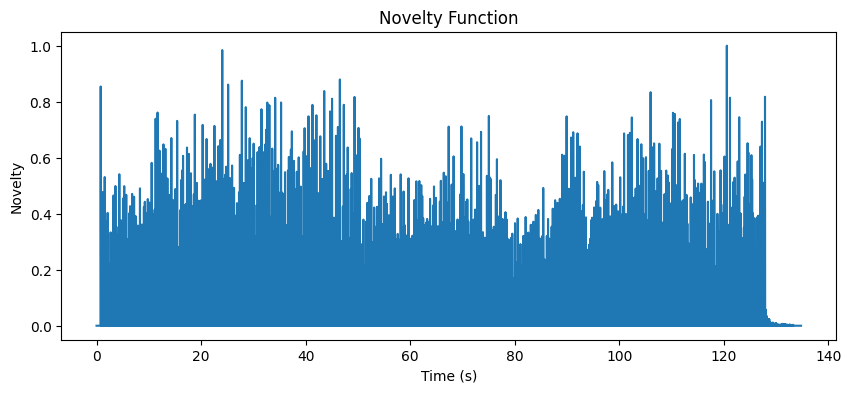
\includegraphics[width=0.5\textwidth]{novelty_3.png}}
    \caption{Novelty curve of the audio track}
    \label{fig:novelty}
\end{figure}
The tempogram representation using Fourier-based method and autocorrelation of the track are shown in Figure \ref{fig:tempogram}, with detected tempos annotated.
\begin{figure}[ht]
    \centering
    \subfloat[Autocorrelation]{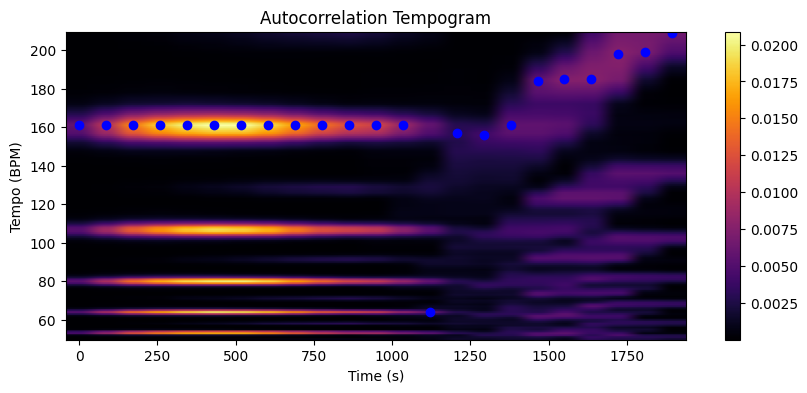
\includegraphics[width=0.5\textwidth]{tempoA_3.png}}
    \subfloat[Fourier-based]{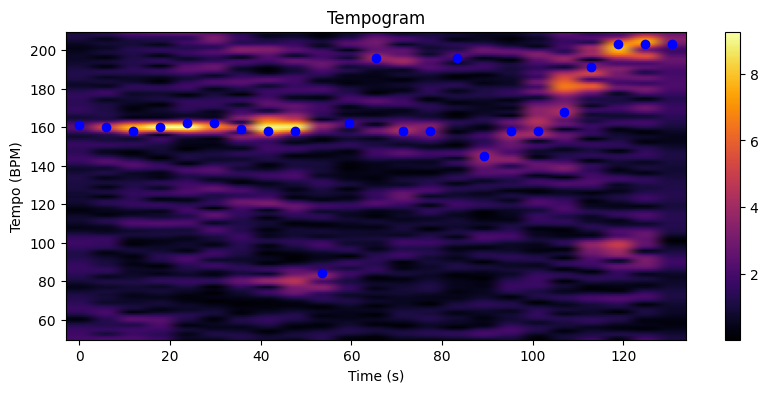
\includegraphics[width=0.5\textwidth]{tempoF_3.png}}
    \caption{Tempogram representation of the audio track}
    \label{fig:tempogram}
\end{figure}
Table \ref{tab:results} shows the global tempo estimation results using both methods, along with the chosen tempo range. Finally, Figure \ref{fig:plp} illustrate the resulting PLP estimation curve on autocorrelation and Fourier tempogram.
\begin{table}
    \centering
    \begin{tabular}{l|c|c}
        \toprule
        \textbf{Track} & \textbf{Tempo (BPM) (ACF)} & \textbf{Tempo range (BPM)} \\
        \midrule
        1 (pop) & 140& [100, 180]\\
        2 (electronic)& 100& [70, 180]\\
        3 (classical)& 161& [50, 210]\\
        \bottomrule
    \end{tabular}
    \caption{Tempo estimation results for the audio track}
    \label{tab:results}
\end{table}
\begin{figure}[bht]
    \centering
    \subfloat[Autocorrelation]{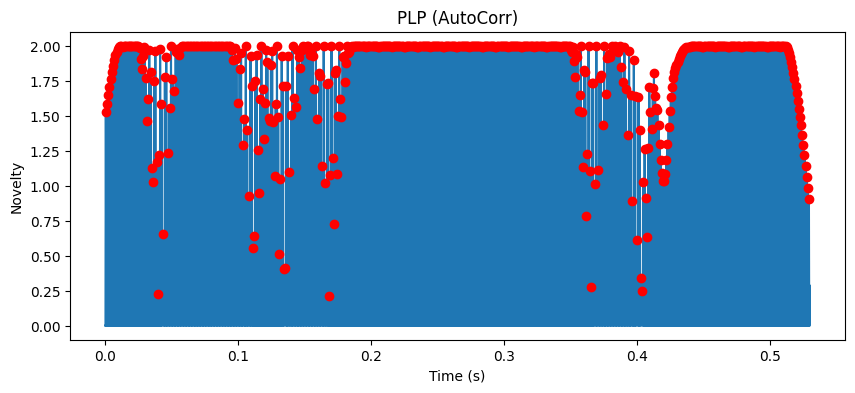
\includegraphics[width=0.5\textwidth]{plpA_3.png}}
    \subfloat[Fourier-based]{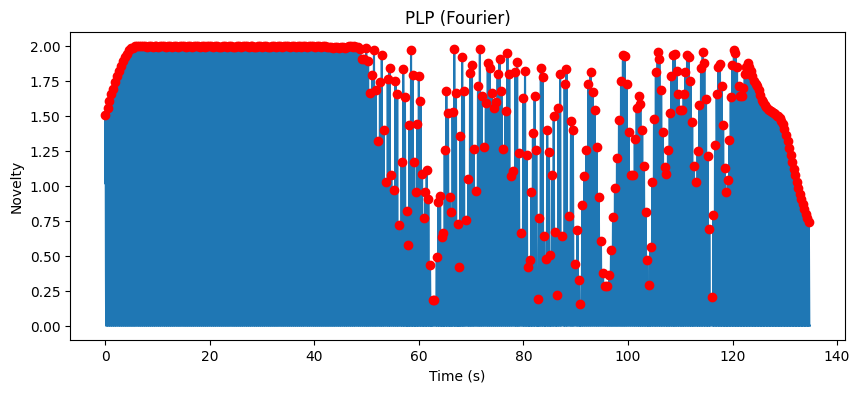
\includegraphics[width=0.5\textwidth]{plpF_3.png}}
    \caption{PLP curve of the audio track}
    \label{fig:plp}
\end{figure}
\section*{Challenges and Solutions}

Several challenges were encountered during the implementation:

\subsection*{Difficulties Encountered}
\begin{enumerate}
    \item \textbf{Detecting Onsets in Non-Percussive Music}: Tracks with subtle or blurred onsets (e.g., classical or jazz music) posed difficulties for onset detection using spectral flux.
    \item \textbf{Tempo Variations}: Handling tempo changes (such as \textit{accelerando} or \textit{ritardando}) was challenging, particularly for tracks with drastic tempo fluctuations.
    \item \textbf{PLP Estimation}: Accurately estimating the \textit{Predominant Local Pulse} in highly dynamic and expressive music was challenging, as small variations in tempo or rhythm can lead to instability in the PLP curve.
\end{enumerate}

\subsection*{Possible Improvements}
\begin{enumerate}
    \item \textbf{Enhanced Onset Detection}: Future improvements could focus on using more advanced onset detection algorithms that better handle non-percussive music, such as those relying on \textbf{machine learning}.
    \item \textbf{Adaptive Tempo Tracking}: Introducing more advanced models, such as \textbf{dynamic time warping (DTW)}, would help improve accuracy in tracking tempo changes over time.
    \item \textbf{Noise Reduction in PLP Estimation}: Smoothing the PLP curve using more sophisticated filters, or employing \textbf{machine learning} to model the predominant pulse, could enhance accuracy in challenging tracks.
\end{enumerate}
\section*{Conclusion}
The project successfully implemented a system for beat tracking and tempo estimation in music signals. Despite several limitations regarding tempo variations, the system managed to accurately estimate the beat and tempo for various music genres, especially during stable tempo sections. Future work could focus on enhancing the system's robustness to tempo variations and improving the accuracy of PLP estimation in expressive music.

\bibliographystyle{IEEEtran}
\bibliography{references}

\end{document}
